\documentclass{standalone}
\usepackage{tikz}
\usepackage{amsmath}
\usepackage{pgfplots}
\usetikzlibrary{calc,positioning,shapes.misc,shapes.multipart}
\begin{document}
	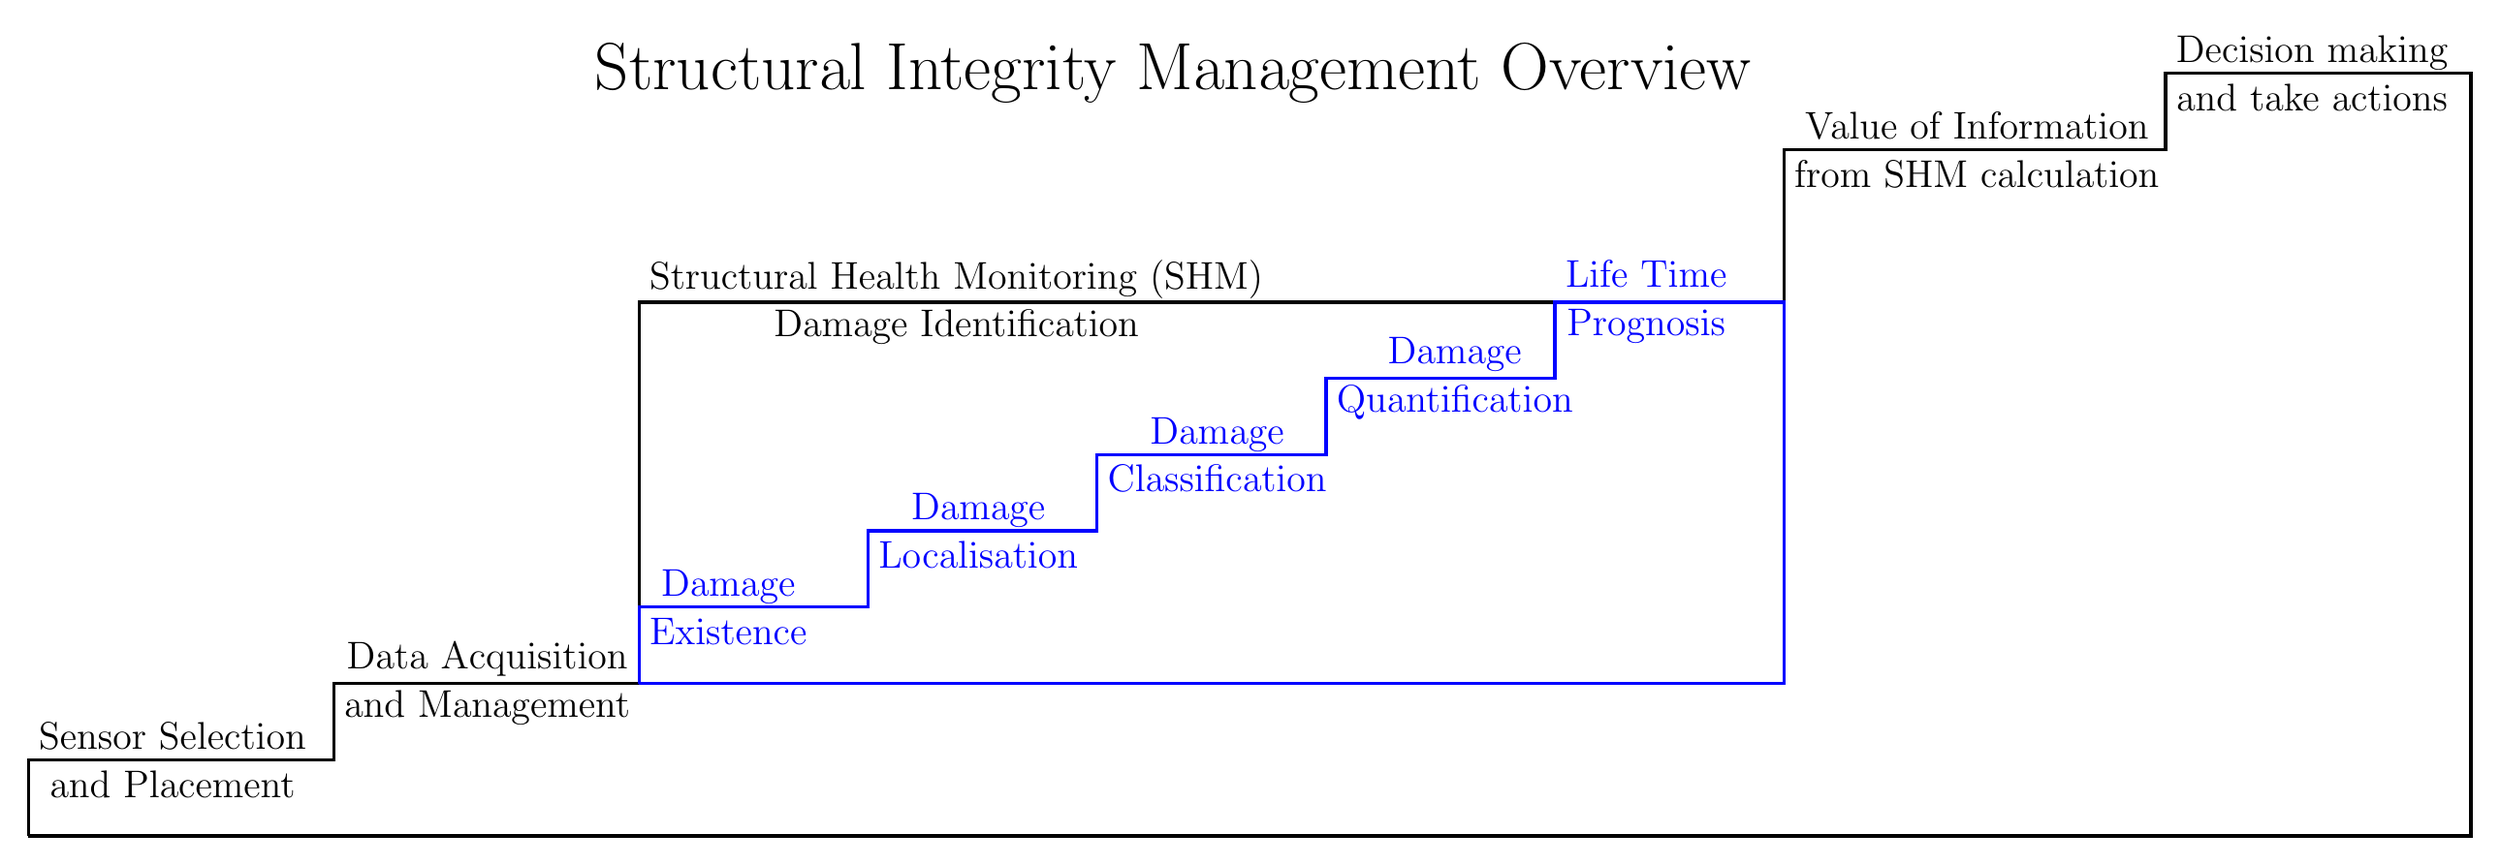
\begin{tikzpicture}[>=latex,every text node part/.style={align=center}]
		\tikzstyle{every node}=[font=\Large];
		\draw[black,very thick] (0,0) -- ++ (0,1)  node [right] {Sensor Selection \\ and Placement} -- ++ (4,0)--++ (0,1) node [right] {Data Acquisition \\and Management}-- ++(4,0) --++ (0,5) node [right] {Structural Health Monitoring (SHM) \\Damage Identification } --++ (15,0) -- ++(0,2) node [right] {Value of Information \\ from SHM calculation} --++ (5,0) --++ (0,1) node [right] {Decision making\\ and take actions}--++(4,0)--++ (0,-10) -- (0,0) ;
		
		\draw[blue,very thick] (8,2) --++ (0,1) node[right]{Damage \\ Existence} --++ (3,0) --++ (0,1)  node[right] {Damage \\ Localisation}--++ (3,0) --++(0,1) node[right]{Damage \\ Classification}--++(3,0) --++ (0,1) node[right] {Damage \\ Quantification} --++ (3,0)--++(0,1) node[right] {Life Time \\ Prognosis} --++ (3,0) --++ (0,-5) -- (8,2);
		
		\draw (15,10) node {\Huge Structural Integrity Management Overview};

	\end{tikzpicture}
\end{document}